\newpage
\section{Ground penetrating radar}

\subsection{Principle}

Ground penetrating radar, or GPR, is a technology to investigate the subsurface using radars. A transmitter (in orange marked Tx on the figure \ref{fig:GPR}) generates an electromagnetic wave which is transmitted into the ground via an antenna. This signal will propagate into the ground at different velocities depending on the material ($0.13 m/ns$ for sandstone or $0.5 m/ns$ for fresh water \cite{GPRAnalysis}) and will be both reflected and transmitted on the interface between two different materials. The reflected part will be received by the reception antenna connected to the receiver (Blue marked Rx on the figure \ref{fig:GPR}).

\begin{figure}[h]
    \centering
    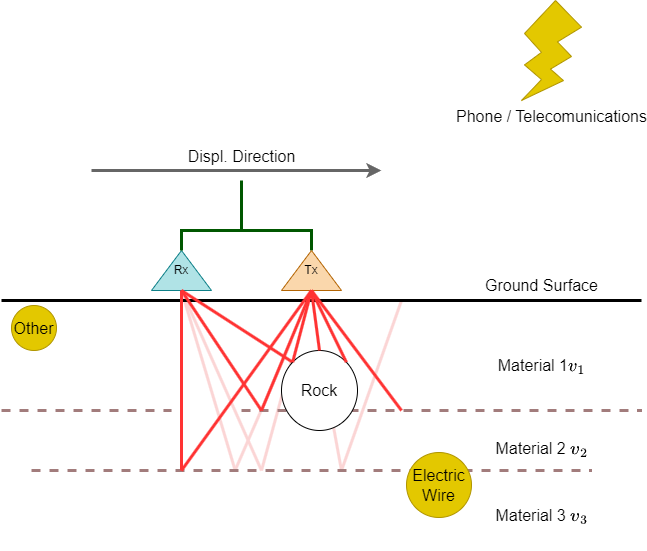
\includegraphics[width=0.8\linewidth]{Images/00_Theory/GPR Diagramm.drawio.png}
    \caption{Ground penetrating radar principle}
    \label{fig:GPR}
\end{figure}

Now that we have the basis of the principles of GPR, we could consider different positioning for both antennae. Indeed, we could choose to keep the receiver fixed and the transceiver moving, at the opposite, both transmitter and receiver moving around a common midpoint... In this report, we will only use the set up with the transmitter and the receiver moving together, antenna perpendicular to the moving direction.
This usage of GPR permits to investigate a big area by doing multiple lines. On each line, each measurement point will represent the ground under the GPR and so we can have an overview of the subsurface along the line. \cite{Rnning2023GroundPerformance}

\subsection{Limitations}

As the GPR uses a range of frequency from Mhz to Ghz which is also the range for many communication and electronics devices, GPR is very sensitive to all radio-electric perturbations. So it must be operated far from any noise source as electric grid, GSM antenna...

An other limitation is that propagation characteristics depend on the material where the electromagnetic wave propagates. Consequently the energy lost by the wave during its propagation depends on the material as well as the velocity. So for the same time window\footnote{Time during the receiver is waiting the wave to come back before emitting a new signal. See \ref{SubSection:settings}}, if the signal propagates fast or slow, the depth where we can see will be changed. Also, a material with a huge attenuation limits the depth of the survey because the signal will lose very quickly the power.

Finally, every saline environments are almost impossible to investigate with GPR because the conductivity of salty water is very good, too good\cite{UnderstandingDetection}.

\subsection{Settings} \label{SubSection:settings}


\paragraph{Tension} The tension gives an indication about the energy given to the emitted signal. The higher the tension is, deeper the signal will propagate but also higher the GPR will disturb the communication devices. The maximum tension allowed for civil survey is $400V$ even if in the past some GPR with a tension of $1000V$ were used. 

\paragraph{Frequency} The frequency is one of the most important parameters for a GPR survey because it defines the resolution of the GPR. Figure \ref{fig:GPRFrequency} shows that the frequency used is the most important factor which affects the resolution. Also, a higher frequency will penetrate less deep than a low frequency for the same wave energy.

\begin{figure}[h]
    \centering
    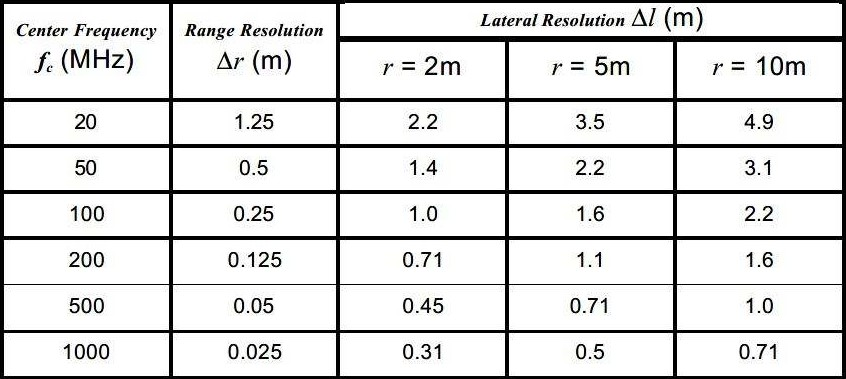
\includegraphics[width=0.6\textwidth]{Images/00_Theory/SS_FrequencyDepthResolution.jpg}
    \caption{Exemple of resolution length and depth versus frequency ($v=0.1m/ns$) from Sensor and Software \cite{UnderstandingDetection}}
    \label{fig:GPRFrequency}
\end{figure}

\paragraph{Number of stacks} The stacking consists in measuring the same data many times to take the medium or mean value and reduce the noise. The number of stacks should be as higher as possible but will depend on the capabilities of the data-logger, of the receiver and on the different other parameters.


\paragraph{Time windows} As defined before, the time window is the time during which the receiver waits for the signal reflected inside the ground. If we use a short time window, we risk to miss information. On the contrary, if the time window is too wide, the data logger will record only noise which will reduce the capability of the data logger.

\paragraph{Sampling interval} The reception antenna received an analog signal coming from the ground but the data-logger only record digital signal. Therefore it is important to have a sampling interval which corresponds to the signal. A sampling interval which is too low will lead a completely different signal. The important criteria is the Nyquist Criteria which indicates that the sampling interval should be smaller than the minimum expected period in order to catch all the expected frequencies.

\begin{figure}[H]
    \centering
    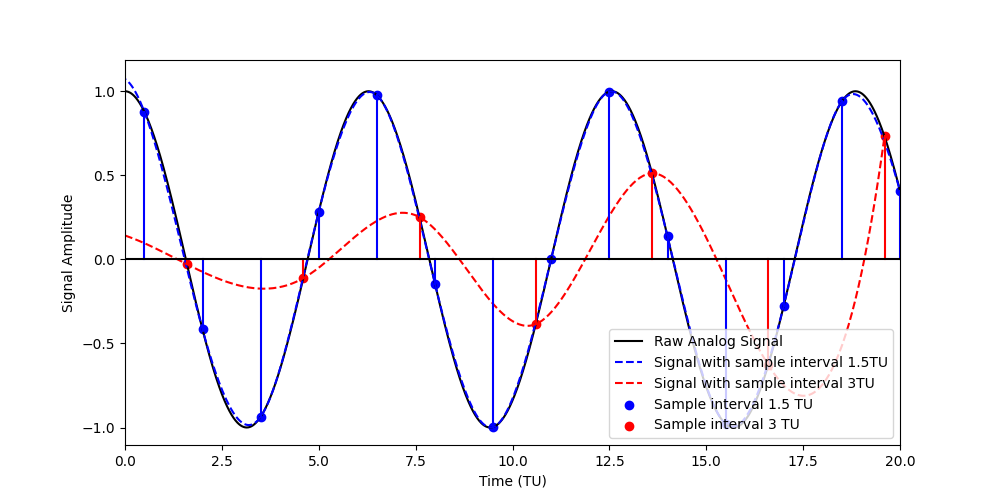
\includegraphics[width=0.8\linewidth]{Images/00_Theory/SampleRate.png}
    \caption{Sample rate illustration}
    \label{fig:SampleRate}
\end{figure}

On the example from figure \ref{fig:SampleRate}, we see that the sample interval of 3 TU\footnote{TU = Time Unit} is too low where the sample interval of 1 TU is better.

\paragraph{Antenna separation} The antenna separation will influence the quality of the signal due to the coupling between the two antennae. In order to set this parameter, we will just refer to the manufacturer documentation.

\paragraph{Antenna orientation} The orientation of both antennae will be chosen for practical purposes : both antennae are perpendicular to the moving direction even if other solutions are possible but leading to a more complicated setting up on the pulk (See \ref{Section:Methodology}). We chose to have the reception antenna the furthest away from any electronic devices.


\paragraph{Sampling distance} The sampling distance will be the distance between two traces, this will give the horizontal resolution. The shorter the distance is, the higher the horizontal resolution will be but also the slower the speed of the displacement will be.

\paragraph{Velocity} The velocity (of displacment of the signal in the ground) is a secondary parameter for a GPR because in many cases the velocity is determined using GPR data. The key thing to know is that the velocity will convert the time window into a depth window defining the depth where the GPR can see.


